\documentclass[12pt]{article}

\usepackage[hmargin=2.5cm, vmargin={3cm,3cm}, a4paper]{geometry} 
\usepackage{amsmath,amssymb,amsthm,mathrsfs}
\usepackage{epsfig,epsf,subfigure,graphicx,graphics}
\usepackage{float}
\usepackage{url,enumerate}
\usepackage{listings}
\usepackage{ragged2e}
\graphicspath{{fig/}}
\usepackage{fancyhdr}
\usepackage{hyperref}
\hypersetup{
    colorlinks=true,
    linkcolor=blue,
    filecolor=magenta,      
    urlcolor=cyan,
    pdfpagemode=FullScreen,
    }
\setlength{\headheight}{12pt}
\pagestyle{fancyplain}

\graphicspath{ {./images/} }%Path to the images
 
\rhead{}
\lhead{}
\chead{{\it Graph Signal Processing Course, ETSETB}}
\lfoot{}
\cfoot{\thepage}
\rfoot{}
\title{Practical session 1: Spectral Clustering}
\author{Gerard Castell and Victor Rubio}
\begin{document}
\maketitle

\thispagestyle{fancyplain}
\flushleft 


\Large
\hspace{10pt}
\small
\section{Mushroom clustering}

%%Abstract Subsection
\subsection{Abstract}
\justifying
The goal of this experiment is to classify a set of mushrooms depending on if they are either edible or poisonous. With that purpose, we will use a dataset experiment which contains 8,124 samples taken from 23 species in the Agarius and Lepiota family. For each sample, there is a label indicating if the mushroom is edible or poisonous and there is also a feature vector detailing a number of its properties such as color, odor and size. In order to solve this classification problem, we will follow a spectral clustering approach to embed the graph nodes into a low-dimensional vector space. Then, k-means is performed on the embedded vectors in order to divide them into clusters.
%%First subsection
\subsection{Reading and cleaning up the data}
\justifying
After downloading the dataset from the \href{https://archive.ics.uci.edu/ml/datasets/mushroom}{UCI website} we found out more information on how the dataset is built. We found that the labeling is classified into edible (e) or poisionous (p) and that there are 2480 missing values (denoted by ''?'') all in the 11\textsuperscript{th} attribute.\\

In order to read and clean the dataset we code the following section to erase such feature from all the mushrooms, hence it is not considered for our experiment:
\smallskip
\begin{lstlisting}[language=matlab]
data = readtable('agaricus-lepiota.txt','ReadVariableNames',false);
data(:,12)=[];

data_label=data(:,1);
data_features=data(:,2:end);

data_label_c = categorical(data_label{:,:});
data_feature_c = categorical(data_features{:,:});
\end{lstlisting}

%Second subsection
\subsection{Feature vector encoding}
\justifying
With the data loaded and cleaned properly, the entries of the features vectors were converted to numerical values using an ordinal encoding:
\smallskip
\begin{lstlisting}[language=matlab]
[~,~, data_feature_vec]=unique(data_feature_c);
data_features_n=reshape(data_feature_vec, size(data_features));

[~,~, data_label_vec]=unique(data_label_c);
data_label_n=reshape(data_label_vec, size(data_label));
\end{lstlisting}

%Third subsection
\subsection{Forming a graph}
\justifying
Once the feature vector encoding was completed we used the \emph{pdist2.m} method to build a weighted graph where each mushroom vector is a node, selecting at first the Hamming distance to calculate the weights:
\smallskip
\begin{lstlisting}[language=matlab]
A = pdist2(data_features_n,data_features_n, 'hamming');

G=graph(A); 
figure(1)
plot(G)
title('Mushrooms Graph')
\end{lstlisting}
\justifying
With the previous code we were able to plot the following  \href{fig:graphRepresentation}{figure} that is the representation of the nodes and weights of the graph. In such a plot we can see clearly that we have built an undirected graph which is fully connected. Each node represents a mushroom sample, so the edges between them are the weight calculated based on the similarity with the Hamming distance, so the intuition of that links is that the bigger the weight is the more similar the mushrooms are. Using this knowledge we have created the similarity matrix, which is the adjacency matrix (A), from that metric of the Hamming distance to end up with a symmetric graph of the samples and now we can apply the Spectral Clustering to classify them.

\begin{figure}[H]
	\centering
	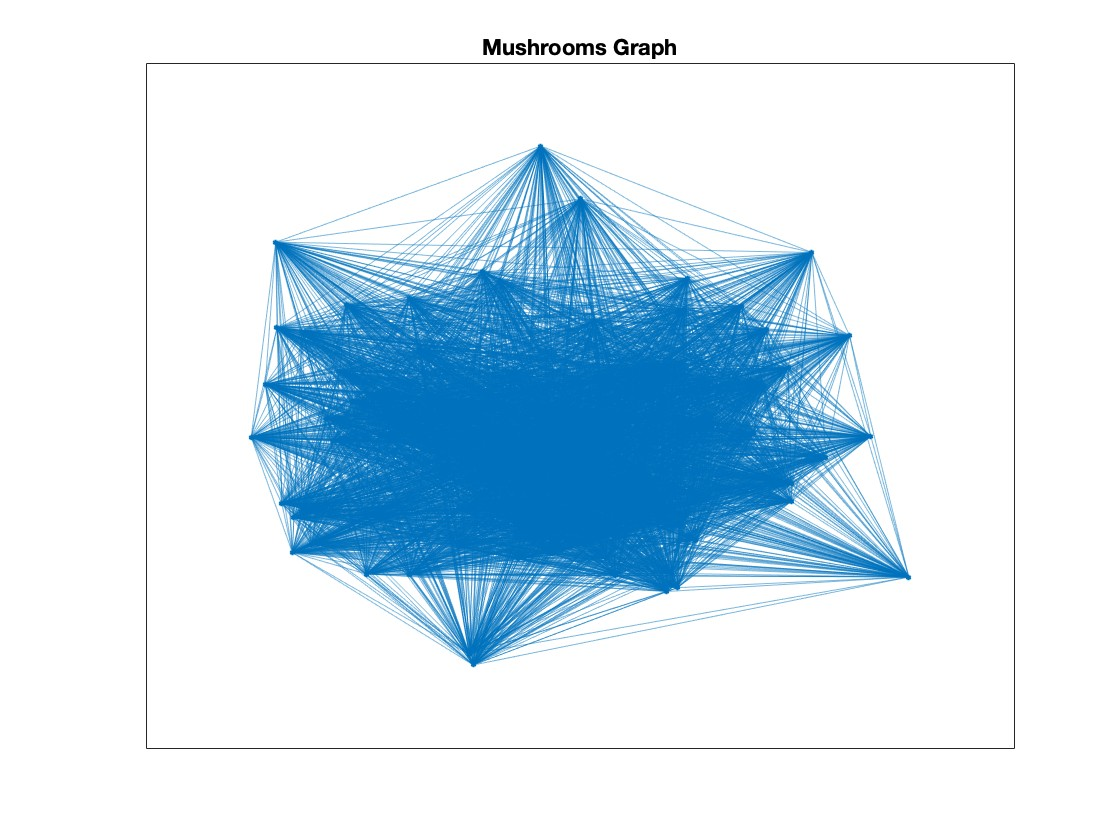
\includegraphics[width=13cm]{1.jpg}
	\caption{Plot of the nodes and edges of the graph built}
	\label{fig:graphRepresentation}
\end{figure}

It is important to note that spectral clustering performance largely depends on the similarity function used to build the graph. So the results obtained in this experiment are closely pegged to the Hamming metric.

%Fourth subsection
\subsection{Spectral clustering}
\justifying
The key concept behind the Spectral Clustering is that \textbf{the multiplicity of the 0 eigenvalue of the Laplacian of a graph is equal to the number of connected clusters} with associated eigenvectors given by the indicator vectors of those clusters. In an ideal world, the graph has k connected or clusters and the Laplacian has an eigenvalue 0 with multiplicity k. The k eigenvectors of the null eigenvalue are linear combinations of the indicator vectors and allow us to identify the nodes of each cluster, which is our main target. However, in a real scenario like the one for this experiment, \textbf{we expect to obtain small eigenvalues of the Laplacian}, which are an approximation of the null eigenvalues of the Laplacian, so the corresponding eigenvectors are an approximation as well of the indicator vectors.

Then, we wanted to embed the graph nodes into a low-dimensional vector space where data points shall be organized according to the graph weights, performing k-means on the embedded vectors in order to divide them into clusters afterwards. We used the normalized graph Laplacian, calculated eigenvalues and eigenvectors and used the first 2 eigenvectors with the k-means function \emph{kmeans.m}:
\smallskip
\begin{lstlisting}[language=matlab]
on=ones(size(A,1),1);
D_vec=(A*on);
D_mat=diag(D_vec);
D_inv2=diag(D_vec.^(-.5));
L=D_mat-A;
nL=D_inv2*L*D_inv2;
[veps,vaps]=eig(nL);
k=2;
idx=kmeans(veps(:,1:2),k);
\end{lstlisting}

%Fifth subsection
\subsection{Performance evaluation}
\justifying
In order to determine the usefulness of the results we compared them to the ground truth using the confusion matrix and calculating the failure probabilities. We also plotted the feature vectors in the embedded space differentiating using colors the different clusters.
\smallskip
\begin{lstlisting}
C=confusionmat(data_label_n, idx);
figure(2)
h=gscatter(veps(:,1), veps(:,2), idx);
title('Scatter plot. Normalized Laplacian. 2 clusters')

figure(3)
h_r=gscatter(veps(:,1), veps(:,2), data_label_n);
title('Sparcification using the real labels')
\end{lstlisting}

\smallskip
\justifying
In order to compare the results we plotted a scatter of the sparcification using the real labels in the figure \href{fig:scatterOriginalLabels}{bellow}. This way we will be able to graphically determine if the model is working properly.

\begin{figure}[H]
	\centering
	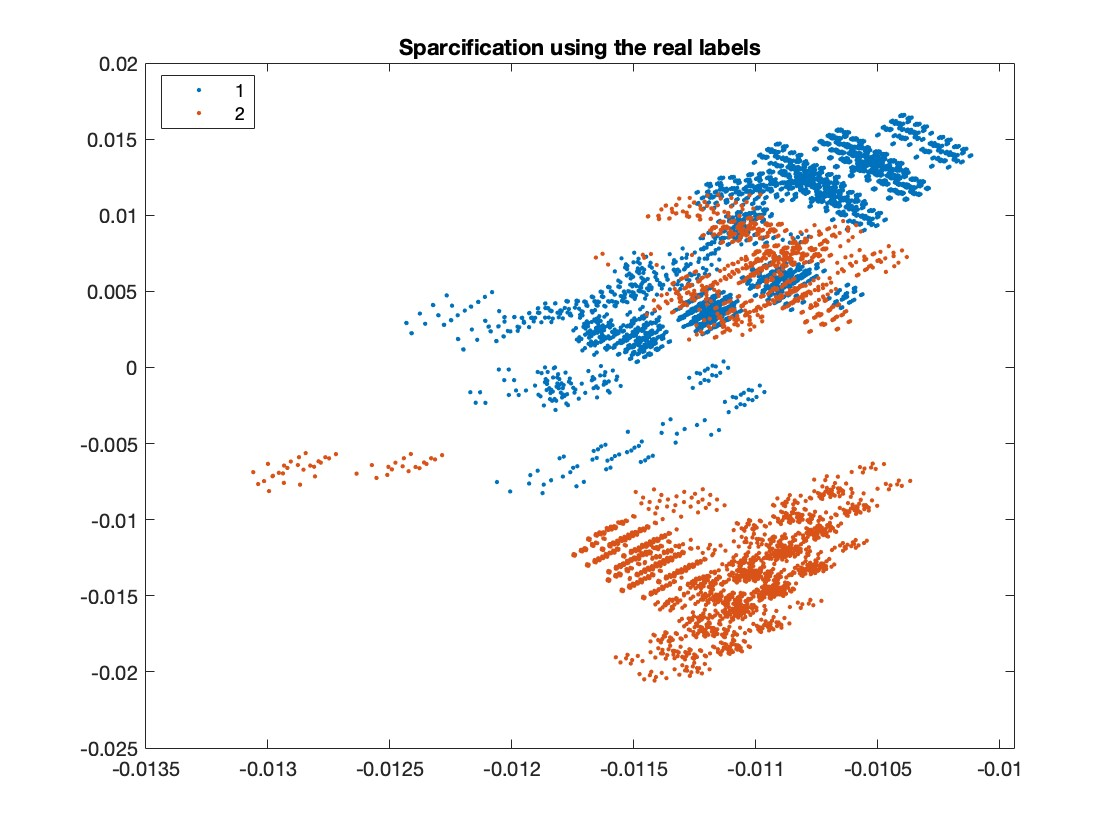
\includegraphics[width=12cm]{3.jpg}
	\caption{Scatter of the data segregated using the real labels}
	\label{fig:scatterOriginalLabels}
\end{figure}


\smallskip
\justifying
Due to our problem, we want to classify mushrooms into edibles or poisonous, we decided to use \emph{k=2} in the k-means to have our samples into two clusters. We used a Normalized Laplacian as discussed previously. In the image \href{fig:normLapl2clusters}{bellow} we can see how these two elements were separated by k-means.

\begin{figure}[H]
	\centering
	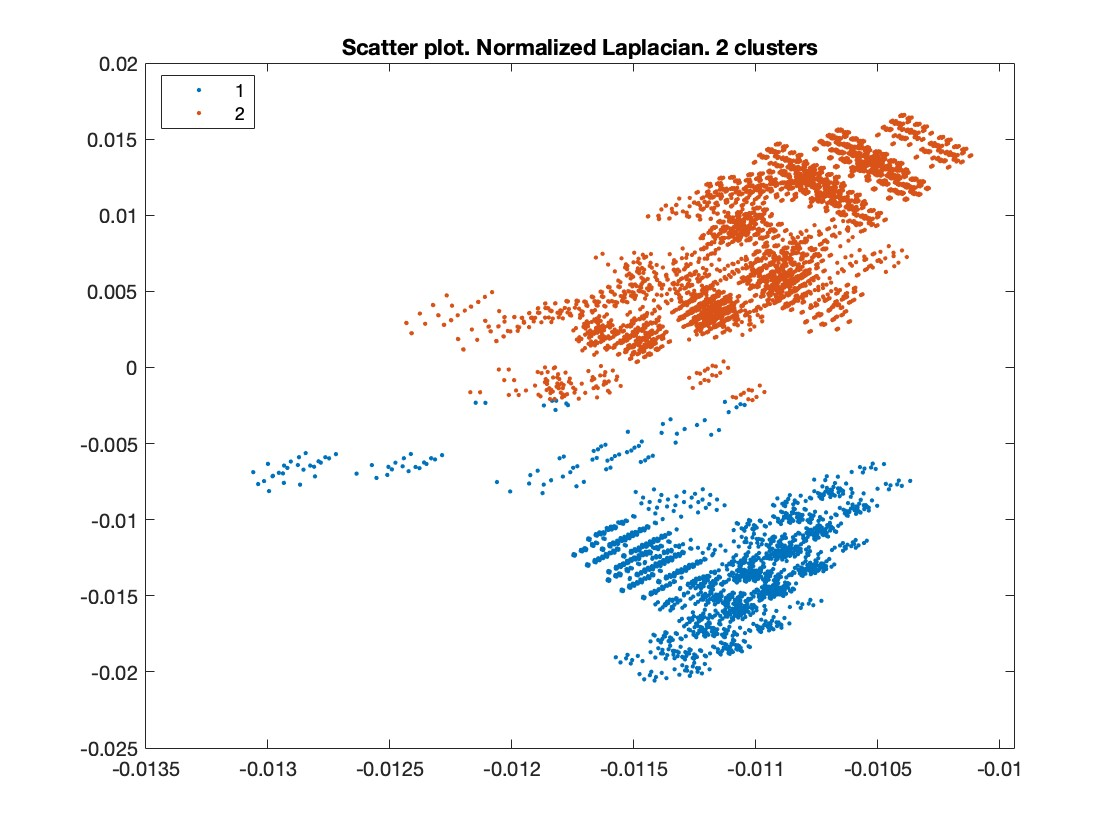
\includegraphics[width=12cm]{2.jpg}
	\caption{Cluster visualization with k=2 and Normalized Laplacian $(L_{sn})$}
	\label{fig:normLapl2clusters}
\end{figure}

\smallskip
\justifying
As you can observe comparing the both images above, there are some samples of one class quite mixed with the other cluster. This confuses the discriminator and makes the task more complicated. The classifier that we obtained clearly has separated all the samples from one class from the other, so we cannot find a mixed samples closely, they are separated almost linearly. As we see, with that approach we are misclassifying that mixed in the other cluster.\\

We also obtained the confusion matrix for the previous configuration:

\begin{figure}[H]
	\centering
	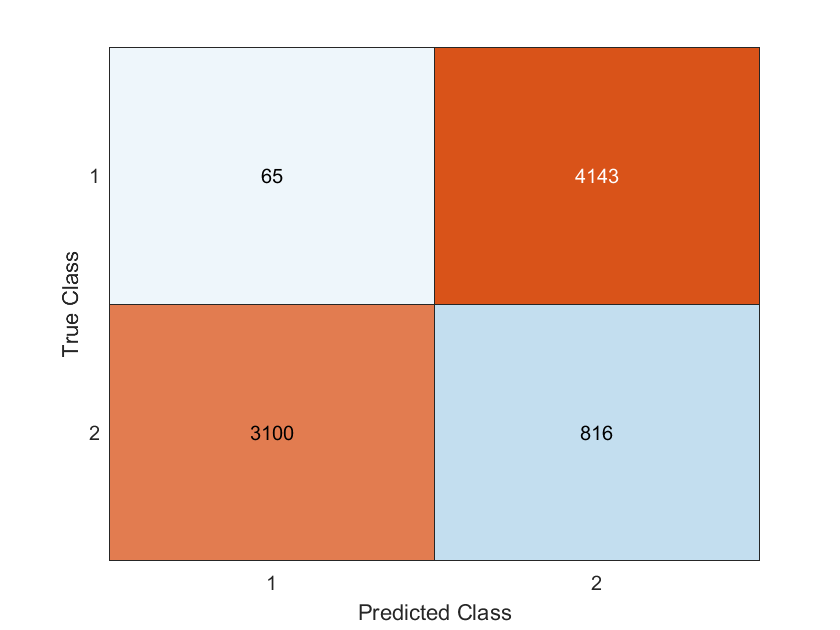
\includegraphics[width=9cm]{confusionk2.png}
	\caption{Confusion matrix of configuration k=2 and Normalized Laplacian $(L_{sn})$}
	\label{fig:confusionk2NormLaplacian}
\end{figure}

So with the aim of find a better segregation results we try using k=3 and recompute the confusion matrix and plot again the results:
\smallskip

\begin{lstlisting}
%% We repeat it with a different number of clusters
k=3;
idx3=kmeans(veps(:,1:3),k);
C3=confusionmat(data_label_n, idx3);
confusionchart(C3);
figure(4)
formats = [".r", ".b", ".g"];

for i = 1:3
    points = veps(idx3 == i, 1:3);
    scatter3(points(:, 1), points(:, 2), points(:, 3), formats(i), 'DisplayName', "Cluster " + i);
    hold on
end

legend('Location', 'Best')
title 'Scatter plot. Normalized Laplacian. 3 clusters'
hold off
\end{lstlisting}

\begin{figure}[H]
	\centering
	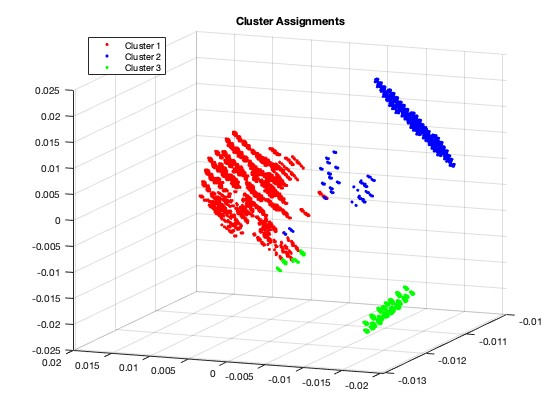
\includegraphics[width=12cm]{3DNormalizedLaplaciank3.jpeg}
	\caption{Cluster visualization with k=3 and Normalized Laplacian $(L_{sn})$ in a 3D view}
	\label{fig:3DnormLapl3clusters}
\end{figure}

\begin{figure}[H]
	\centering
	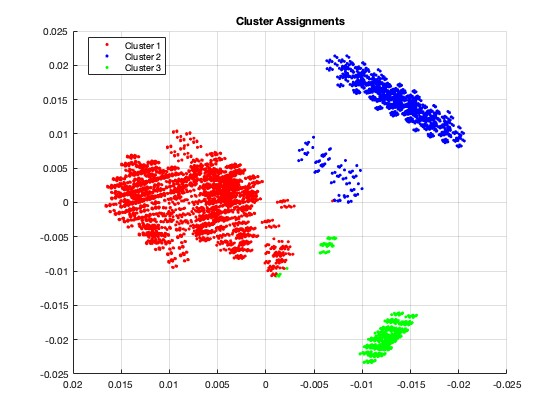
\includegraphics[width=9cm]{2DNormalizedLaplaciank3.jpeg}
	\caption{Cluster visualization with k=3 and Normalized Laplacian $(L_{sn})$ in a 2D view}
	\label{fig:2DnormLapl3clusters}
\end{figure}
As we may observe in the \href{fig:3DnormLapl3clusters}{previous figure}, three clusters are clearly visible, which have been projected onto the the first three eigenvectors as axis and also onto the second and third coordinates in the eigenvector basis.
We compute the confusion matrix again for this configuration:
\smallskip
\begin{figure}[H]
	\centering
	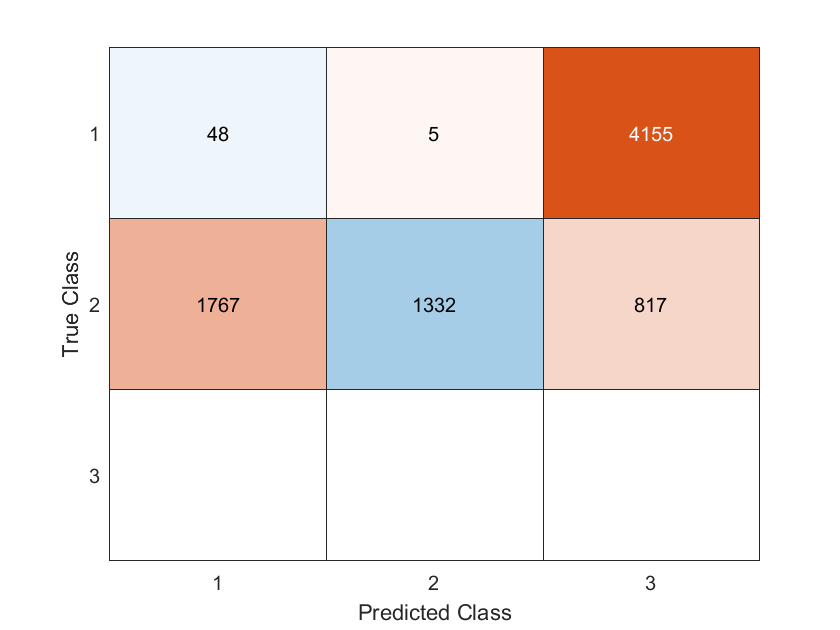
\includegraphics[width=9cm]{confusionk3.png}
	\caption{Confusion matrix of configuration k=3 and Normalized Laplacian $(L_{sn})$}
	\label{fig:confusionk3NormLaplacian}
\end{figure}
\smallskip
\justifying
With the previous confusion matrix we can see that the correct predictions have increased when increasing the number of eigenvectors used.

%Sixth subsection
\subsection{Alternative embeddings and graph sparsification}
\justifying
After adapting the k value in k-means we also wanted to try to classify the elements introducing different embeddings. We used the Unnormalized Laplacian at first, using the first two eigenvalues, although the result was worse than the one we obtained from the normalized laplacian:
\smallskip
\begin{figure}[H]
	\centering
	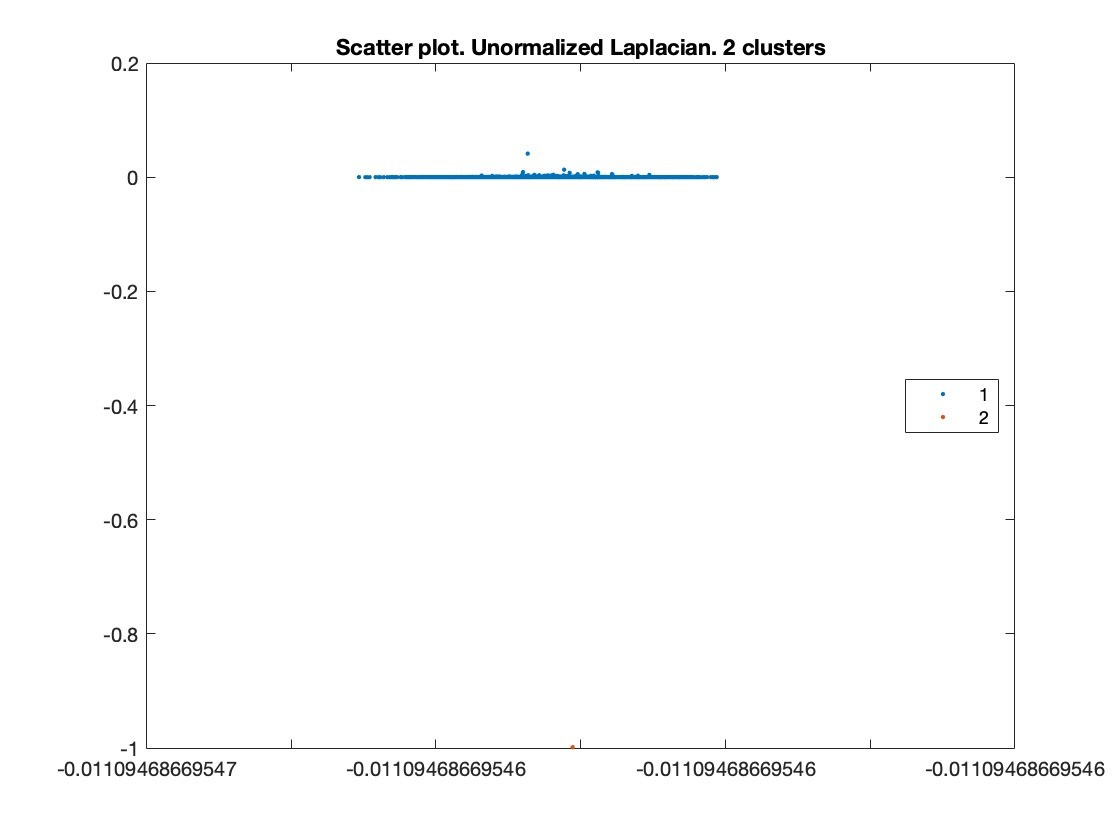
\includegraphics[width=12cm]{5.jpg}
	\caption{Cluster visualization with k=2 and Unnormalized Laplacian $(L)$}
	\label{fig:Lapl2clusters}
\end{figure}
\smallskip
\justifying
In this case we can see that is has only been able to classify one mushroom as poisonous. If we look at the confusion matrix it is evident that the results are worse:
\smallskip
\begin{figure}[H]
	\centering
	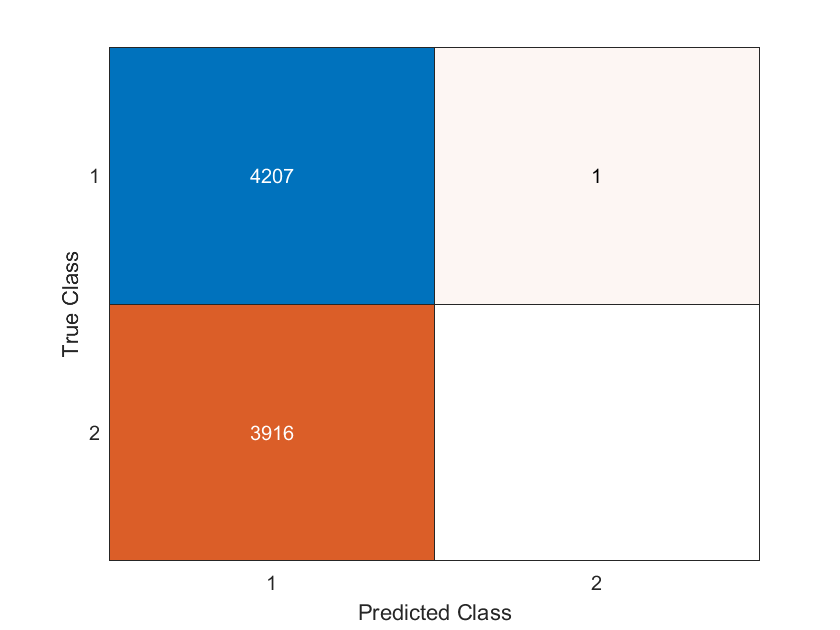
\includegraphics[width=7cm]{confusionL.png}
	\caption{Confusion matrix of configuration k=2 and Unnormalized Laplacian $(L)$}
	\label{fig:confusionL}
\end{figure}

\smallskip
\justifying
Finally we also computed the Random-Walk Laplacian Matrix and using the first two eigenvalues with k-means we plot the following \href{fig:RWLapl2clusters}{figure}: 
\smallskip
\begin{lstlisting}
D_inv=diag(1./D_vec);
rwL=D_inv*L;
[veps_rw,vaps_rw]=eig(rwL);
k=2;
idx_rw=kmeans(veps_rw(:,1:2),k);
figure(6)
h_rw=gscatter(veps_rw(:,1), veps_rw(:,2), idx_rw);
title('Scatter plot. Random-walk Laplacian. 2 clusters')
\end{lstlisting}
\smallskip
\begin{figure}[H]
	\centering
	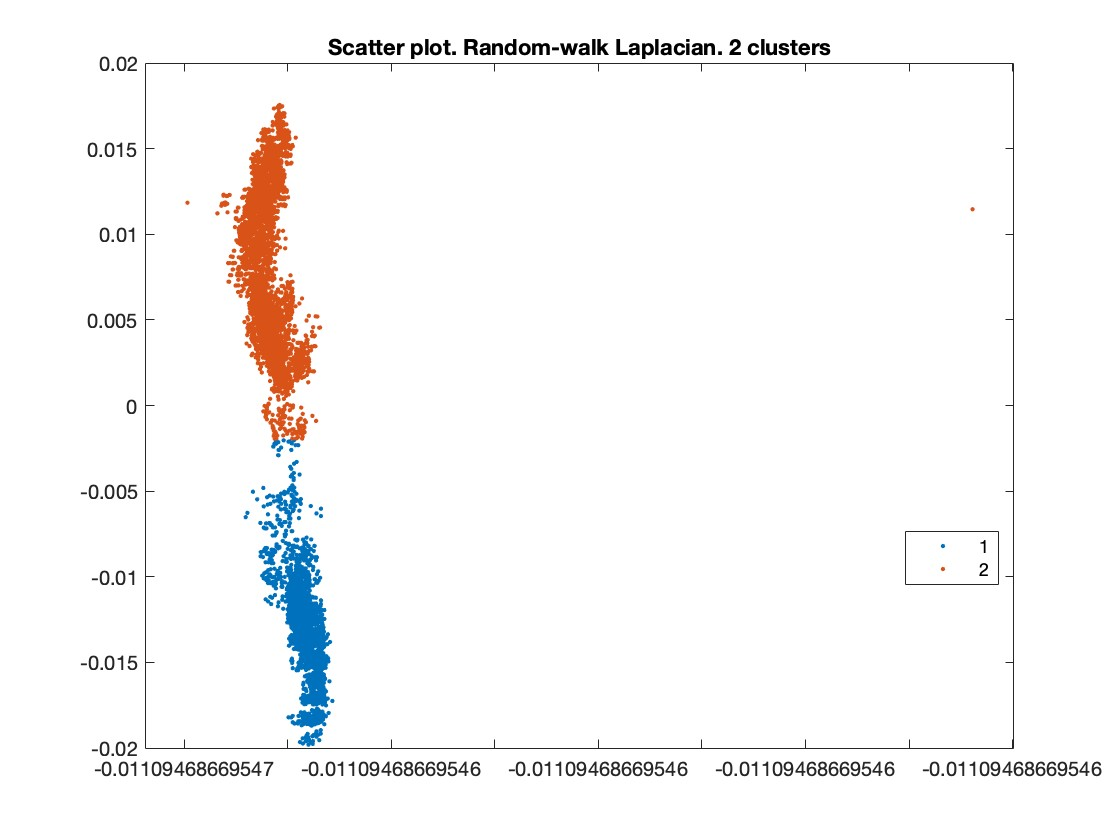
\includegraphics[width=12cm]{6.jpg}
	\caption{Cluster visualization with k=2 and Random-Walk Laplacian $(L_{RW})$}
	\label{fig:RWLapl2clusters}
\end{figure}
\smallskip
\justifying
If we look at the confusion matrix for this configuration we can observe that the result has greatly improved as the amount of correct predictions outweighs the amount of false predictions. This model still can be improved because if we want to detect poisonous mushrooms the false positives should be significantly lower as to avoid risking lives.

\begin{figure}[H]
	\centering
	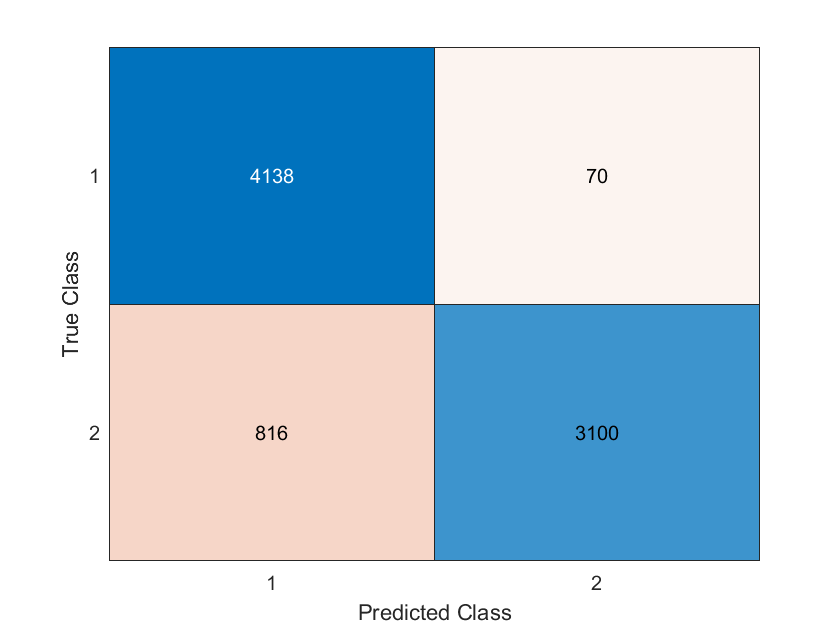
\includegraphics[width=9cm]{confusionLrw.png}
	\caption{Confusion matrix for configuration k=2 and Random-Walk Laplacian $(L_{RW})$}
	\label{fig:confusionLrw}
\end{figure}

\end{document}